\documentclass[czech, american]{article}

%%% Packages
%% Encoding, paper settings, etc.
\usepackage[T1]{fontenc}			% Font encoding
\usepackage[utf8]{inputenc}			% Input encoding
\usepackage[a4paper]{geometry}		% Use of the A4 page

%% Languages
\usepackage[czech, american]{babel}							 % Czech and American English are used in this document
\usepackage{silence}										 % Silence output of warnings
\WarningFilter{biblatex}{File 'american-iso.lbx' not found!} % Silence weird message that I couldn't find a solution for

%% Fonts
\usepackage{amsmath}				% Advanced mathematics package
\usepackage{csquotes}				% Ensure that quoted texts are typeset according to the rules of the main language
\usepackage{soul}					% Text fonts syllable by syllable - used for in-text codifying
\usepackage[hidelinks]{hyperref}	% Hide border around URL links
\hypersetup{
	colorlinks=true, citecolor=blue, filecolor=blue, linkcolor=blue,
	urlcolor=blue
}

%% Graphics
\usepackage{tikz}					% Visual representation of matrices, graphs etc.
\usetikzlibrary{
	external,							% Externalize tikz pictures to avoid recompiling them with every compilation
	positioning
}
\tikzexternalize[					% Add '-shell-escape' to the pdflatex compilation command. In TeXstudio: Options -> Configure Texstudio... -> Commands -> PdfLaTeX: 'pdflatex --synctex=1 -interaction=nonstopmode -shell-escape %.tex'
prefix=images/tikz/,				% Place externalized TikZ-generated images in a specific folder - ignored by git
]
\usepackage{pgfplots}				% For visualizations, graphics, etc.
\pgfplotsset{compat=1.3}			% Use pgfplots version 1.3 specifically

%% Code:
\usepackage{listings} 				% Code formatting package

%% Referencing
\usepackage[
	backend=biber,								  		  	% In TeXstudio, the backend here must correspond to: Options -> Configure TeXstudio... -> Build -> Default Bibliography Tool
	style=iso-numeric,
	sorting=none,
	giveninits=true
]{biblatex}								% Bibliography: ISO 690 format, cite shows numbers, sort according to occurrence in the text, shorten first names
\addbibresource{contents/bibliography.bib}				  	% Specify path to bibliography file
\DeclareFieldFormat{labelnumberwidth}{\mkbibbrackets{#1}}	% Square brackets around numbers in the bibliography
\DeclareFieldFormat*{citetitle}{\mkbibemph{#1}}				% \citetitle{bibid} in text produces the title in emphasis for all sources. Without this, for example, the 'thesis' citation entry is non-emphasized with quotes while online sources are only emphasized (looks bad)
\setcounter{biburllcpenalty}{7000}						  	% Insert breakpoints after lowercase letters in URLs in the bibliography
\setcounter{biburlucpenalty}{8000}						  	% Insert breakpoints after uppercase letters in URLs in the bibliography
\DeclareCiteCommand{\citeauthor}							% Custom format of citeauthor: 'J. H. Watson`
{\boolfalse{citetracker}%
	\boolfalse{pagetracker}%
	\usebibmacro{prenote}}
{\ifciteindex
	{\indexnames{labelname}}
	{}%
	\printnames[given-family]{labelname}}
{\multicitedelim}
{\usebibmacro{postnote}}

%% Document settings
\parindent=0pt 		   % Indentation of the 1st line of the paragraph
\parskip=7pt   		   % Space between paragraphs

%%% Custom colors
\definecolor{gray-light}{gray}{0.95}			% Inline code highlighting color
\definecolor{lbcolor}{rgb}{0.9,0.9,0.9}			% Code block background color

%%% Custom code block
\lstset{
	backgroundcolor=\color{lbcolor}, % Background color of the code block
	upquote=true,					 % Format of quote: true -> '', false -> ‘’
	columns=fixed,					 % Characters are below each other (each column is one character -> fixed column size)
	extendedchars=false,			 % Allow national characters, for example, Czech diacritics. If true, then load any package that defines the characters, for example, fontenc, or inputenc, etc.
	showtabs=false,					 % Tabulators visible or not
	showspaces=false,				 % All blank spaces visible as _ or not
	showstringspaces=false,			 % Blank spaces in strings visible as _ or not 
	identifierstyle=\ttfamily,		 % Code font to be monospace if the line begins with one of the following: a-z, A-Z, @, $ and _
	language=Python,				 % Default language syntax highlighting for code blocks
	captionpos=b,					 % Position of the caption. b - bottom; t - top of the listing
	tabsize=2,						 % Set tabulator stops			
	frame=lines,					 % Draw a line on the top and bottom of the code listing -> frame
	numbers=left,					 % Print line numbers on the left of the code block
	numberstyle=\tiny,				 % Font and size of line numbers
	numbersep=5pt,					 % Distance between line numbers and the code block
	basicstyle=\footnotesize,		 % Basic font. Selected at the beginning of each listing
	keywordstyle=\color[rgb]{0,0,1}, % Fond of language keywords in a specific font
	commentstyle=\color{green-dark}, % Font of comments in code block
	stringstyle=\color{red},		 % Font of non-keywords, comments and strings
	breaklines=true,				 % Breaking of long lines
	prebreak = \raisebox{0ex}[0ex][0ex]{\ensuremath{\hookleftarrow}}, % Line-break symbol if a line of code is too long
}

%%% Custom commands
\DeclareRobustCommand{\code}[1]{{\begingroup\sethlcolor{gray-light}\hl{\texttt{#1}}\endgroup}} % Shortcut for code font in text
\soulregister{\code}{1}																		   % Codeify inline text character by character

%%% String variables
\newcommand{\Author}{Lukáš Matthew Čejka}
\newcommand{\Institute}{FNSPE CTU in Prague}
\newcommand{\Date}{\today}
\newcommand{\ProtocolSubTitle}{Heuristic Algorithms - Assessment Task Protocol}
\newcommand{\ProtocolTitle}{Analysis of Heuristics Methods for Acitivity Dependency Problems}

\begin{document}

\title{\ProtocolSubTitle \\
\textbf{\ProtocolTitle}}
\author{\Author}
\maketitle

%%%%%%%%%%%% CONTENTS OF THE PAPER %%%%%%%%%%%%
\selectlanguage{american}
{
	\hypersetup{linkcolor=black}
	\tableofcontents
}

%--------------------------------------------------------
%|         The PAPER ITSELF begins here                 |
%--------------------------------------------------------

\newpage

\section{Introduction}
The development of large-scale projects often requires vast resources, however, the resources available are often limited.
Therefore, completing projects with limited resources before a deadline requires meticulous planning.
Specifically, the resources available at any point in time must be utilized as efficiently as possible.
This goal is one of the key aspects of project management and scheduling.

Many methods that aid in planning the activities of a project with limited resources exist; referred to as \textit{activity dependency problems} in this protocol.
Among the most well-known methods is the Critical Path Method (CPM) \cite{Kelley1959} introduced by \citeauthor{Kelley1959}.
Other methods include heuristics such as those presented in \citetitle{Fiala2008} \cite{Fiala2008}.
While these methods are predominantly used in project management, they can also be used to plan jobs of a data-processing engine.
For this purpose, the protocol aims to introduce a selection of heuristic methods and compare them on a set of problems.

First, the theory behind the heuristic methods is introduced.
Next, the implementation done as part of the assessment project is briefly described.
Then, the results of the comparison of the heuristic methods across several problems is presented.
Finally, the last section summarizes the contents of this protocol.


\section{Theory}

\setcounter{footnote}{3} % Workaround for using footnotemark in theory.tex
\section{Implementation}
In this section, the implementation of the project comprising the methods introduced in Section~\ref{Section:theory} is presented.
The source code is available on request or in the project's GitHub repository\footnote{Heuristic Methods for Activity Dependency Problems GitHub repository URL: \url{https://github.com/CejkaLuk/heuristics-task-dependency}}.
The project was implemented in Python (version 3.9.6\footnote{Python 3.9.6 available at: \url{https://www.python.org/downloads/release/python-396}}) as it offers clean data structures and support for visualization tools.

The project uses the following \textit{make}\footnote{GNU Make webpage URL: \url{https://www.gnu.org/software/make}} tasks:

\begin{tight_itemize}
	\item \code{make init} - Download and install the required Python packages.
	\item \code{make tests}, \code{make tests\_coverage}, and \code{make tests\_coverage\_report} - Run the unit tests using \textit{nose2}\footnote{Nose2 testing framework webpage URL: \url{https://docs.nose2.io/en/latest}} alone, with coverage, and with coverage generated into an HTML report, respectively.
	\item \code{make docs} (executed in \code{docs/}) - Generate the project documentation using \textit{Sphinx}\footnote{Sphinx documentation generator webpage URL: \url{https://www.sphinx-doc.org/en/master}}.
	\item \code{make clean} (executed in the repository root or in \code{docs/}) - Clean the generated files.
\end{tight_itemize}

The core functions of SHM, PHM, and PHMDP are presented in Listings~\ref{Listing:implementation->shm->solve-function}, \ref{Listing:implementation->phm->solve-function}, and \ref{Listing:implementation->phmdp->solve-function}, respectively.

\begin{lstlisting}[caption={The core functions of SHM: \code{solve()} and \code{\_schedule\_activity()}. Note that unimportant functions have been omitted for brevity.},label={Listing:implementation->shm->solve-function}]
def solve(self):
"""Solves the activity dependency problem with resources."""
	
	self.cpm.solve()
	
	# Schedule activities
	for act in self.cpm.project.activities:
		self._schedule_activity(act)
	
	self.cpm.project.actual_end = self._get_project_actual_end()
	
def _schedule_activity(self, act: Activity):
	"""Schedules an activity as soon as possible considering dependencies and available resources."""

	# Get the time when all precessors of act have been completed
	time = self._get_predecessors_finished_time(act)
	
	while not act.is_scheduled():
		tentative_act_end = time + act.duration
		
		# Get the time when the available resources are exceeded between 'time' and 'tentative_act_end'
		time_resources_exceed = self._get_time_available_resources_exceeded(act, time, tentative_act_end)
		
		# If the resources are not exceeded in the time frame, then schedule the activity from 'time'
		if time_resources_exceed is None:
			self._schedule_activity_from(act, time)
		# Otherwise proceed to the next time when the resources are not exceeded
		else:
			time = time_resources_exceed + 1
\end{lstlisting}

\begin{lstlisting}[caption={The core function of PHM: \code{solve()}.},label={Listing:implementation->phm->solve-function}]
def solve(self):
	"""Solves the activity dependency problem with resources and time reserves as priorities."""
	
	self.cpm.solve()
	
	self._init_activity_priorities()
	
	time = 0
	while self._unfinished_activities_exist(time):
		# For PHM, this function does nothing, it serves as a placeholder so that PHMDP can reuse the 'solve' function
		self._update_priorities(time)
		
		# Get activities that can be schedule from 'time'
		viable_activities = self._get_viable_activities(time)
		
		if len(viable_activities) > 0:
			self._sort_by_priority_and_id(viable_activities)
			
			# Try to schedule all viable activities if they don't exceed the available resources
			for act in viable_activities:
				if not self._resources_exceeded(act, time, time + act.duration):
					self._schedule_activity_from(act, time)
		
		# Jump to the next time when an activity finishes as that is when more activities can be scheduled
		time = self._get_time_next_act_finish(time)
	
	self.cpm.project.actual_end = self._get_project_actual_end()
\end{lstlisting}

\begin{lstlisting}[caption={The core functions of PHMDP. The PHMDP class inherits from PHM, therefore, it only overrides functions that deal with priorities.},label={Listing:implementation->phmdp->solve-function}]
def _init_activity_priorities(self):
	"""Override the method in PHM to avoid initializing activities without time."""

def _update_priorities(self, time: int):
	"""Override the method in PHM to update the priorities dynamically."""
	for act in self.cpm.project.activities:
		act.priority = act.latest_start - time
\end{lstlisting}

\section{Comparison}
This section presents the results of the comparison of the heuristic methods presented in Section~\ref{Section:theory}.
While the heuristics were compared on thousands of problems, only the results of four are presented in this protocol due to trade secrets.
Specifically, the methods were compared across four real-life scheduling problems obtained from a data-processing engine.
The problems contained between 7 and 12 activities, and the resources corresponded to the number of CPU cores available to the engine.
One problem was presented in Section~\ref{Section:theory}, and three problems are presented in this section.

For each problem, the CPM network is presented.
In this section, the edges representing jobs in the CPM networks have two values associated with them: computation time in seconds and CPU cores required.

\subsection{Problem 1}
The visualization of problem 1 as a CPM network is shown in Figure~\ref{Figure:comparion->problem->1->cpm-network}. For this problem, $r_\mathrm{max}$ was set to 7.

\begin{figure}[ht!]
	\centering
	\begin{tikzpicture}[
		mynode/.style={
			circle,
			draw=black,
			fill=gray,
			fill opacity = 0.3,
			text opacity=1,
			inner sep=0pt,
			minimum size=20pt,
			font=\small},
		myarrow/.style={-Stealth},
		node distance=0.6cm and 1.2cm
		]
		\node[mynode] (n1) {1};
		\node[mynode,above right=of n1] (n2) {2};
		\node[mynode,below=of n2] (n3) {3};
		\node[mynode,below=of n3] (n4) {4};
		\node[mynode,right=of n3] (n5) {5};
		\node[mynode,right=of n5] (n6) {6};
		
		\foreach \i/\j/\txt/\p in {% start node/end node/text/position
			n1/n2/{4, 3}/above,
			n1/n3/{6, 5}/above,
			n1/n4/{5, 4}/above,
			n2/n5/{3, 3}/above,
			n3/n5/{4, 3}/above,
			n4/n6/{4, 5}/below,
			n5/n6/{3, 3}/above}
		\draw [myarrow] (\i) -- node[sloped,font=\small,\p] {\txt} (\j);
		
	\end{tikzpicture}
	\caption{Visualization of problem 1 as a CPM network.
		Each weighted edge represents a job, its duration (in seconds), and the number of CPU cores required.
	}
	\label{Figure:comparion->problem->1->cpm-network}
\end{figure}

The timelines produced by SHM, PHM, and PHMDP are shown in Figures~\ref{Figure:comparison->problem->1->timelines->shm}, \ref{Figure:comparison->problem->1->timelines->phm}, and \ref{Figure:comparison->problem->1->timelines->phmdp}, respectively.
As can be seen from the figure, unexpectedly, PHM produced the best results for this problem as it scheduled the jobs to be completed within 20 seconds.
However, PHMDP was only one second behind.
This is due to the dynamic priorities holding back certain jobs, such as 1-4, even though they need not have been.

\begin{figure}[ht!]
	\centering
	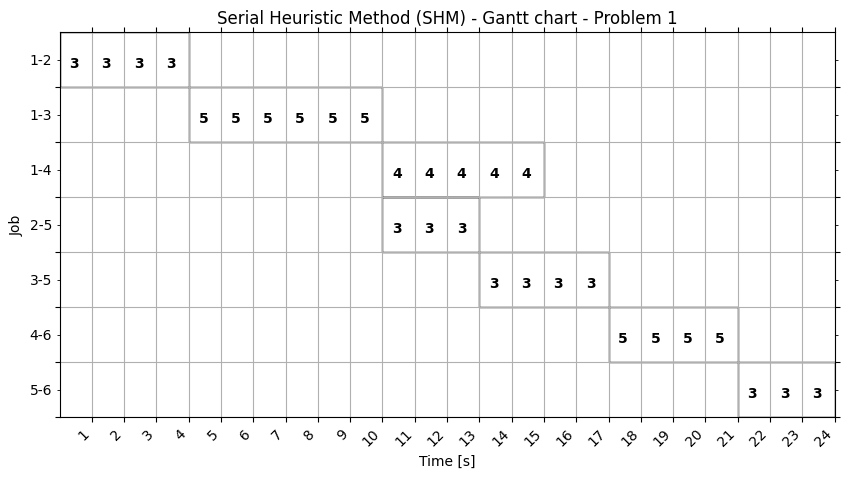
\includegraphics[width=0.7\linewidth]{images/comparison/shm_problem_1.png}
	\caption{Timeline of the activities in problem 1 as scheduled by SHM.
		The vertical axis represents the job, while the horizontal axis displays the time in seconds.
		The numbers in the squares represent the CPU cores required by each job at a point in time.
	}
	\label{Figure:comparison->problem->1->timelines->shm}
\end{figure}

\begin{figure}[ht!]
	\centering
	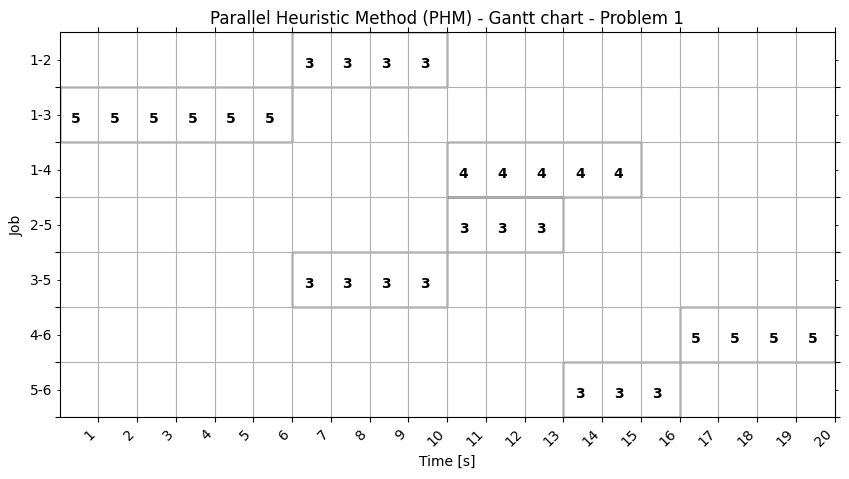
\includegraphics[width=0.7\linewidth]{images/comparison/phm_problem_1.png}
	\caption{Timeline of the activities in problem 1 as scheduled by PHM.}
	\label{Figure:comparison->problem->1->timelines->phm}
\end{figure}

\begin{figure}[ht!]
	\centering
	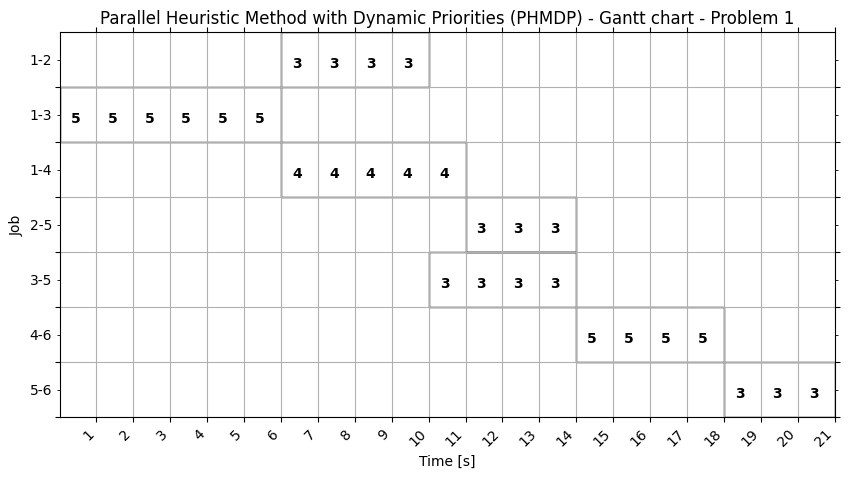
\includegraphics[width=0.7\linewidth]{images/comparison/phmdp_problem_1.png}
	\caption{Timeline of the activities in problem 1 as scheduled by PHMDP.}
	\label{Figure:comparison->problem->1->timelines->phmdp}
\end{figure}

\subsection{Problem 2}
The visualization of problem 2 as a CPM network is shown in Figure~\ref{Figure:comparion->problem->2->cpm-network}. For this problem, $r_\mathrm{max}$ was set to 8.

\begin{figure}[ht!]
	\centering
	\begin{tikzpicture}[
		mynode/.style={
			circle,
			draw=black,
			fill=gray,
			fill opacity = 0.3,
			text opacity=1,
			inner sep=0pt,
			minimum size=20pt,
			font=\small},
		myarrow/.style={-Stealth},
		node distance=0.6cm and 1.2cm
		]
		\node[mynode] (n1) {1};
		\node[mynode,above right=of n1] (n2) {2};
		\node[mynode,below right=of n1] (n3) {3};
		\node[mynode,below right=of n2] (n4) {4};
		\node[mynode,above right=of n4] (n5) {5};
		\node[mynode,below right=of n4] (n6) {6};
		\node[mynode,below right=of n5] (n7) {7};
		
		\foreach \i/\j/\txt/\p in {% start node/end node/text/position
			n1/n2/{5, 3}/above,
			n1/n3/{6, 4}/above,
			n1/n4/{10, 3}/above,
			n2/n4/{1, 3}/above,
			n2/n5/{6, 2}/above,
			n3/n4/{2, 3}/above,
			n3/n6/{5, 3}/above,
			n4/n5/{8, 3}/below,
			n4/n6/{7, 2}/below,
			n5/n6/{9, 4}/above,
			n5/n7/{7, 4}/above,
			n6/n7/{12, 4}/above}
		\draw [myarrow] (\i) -- node[sloped,font=\small,\p] {\txt} (\j);
		
	\end{tikzpicture}
	\caption{Visualization of problem 2 as a CPM network.
		Each weighted edge represents a job, its duration (in seconds), and the number of CPU cores required.
	}
	\label{Figure:comparion->problem->2->cpm-network}
\end{figure}

The timelines produced by SHM, PHM, and PHMDP are shown in Figures~\ref{Figure:comparison->problem->2->timelines->shm}, \ref{Figure:comparison->problem->2->timelines->phm}, and \ref{Figure:comparison->problem->2->timelines->phmdp}, respectively.
In the case of problem 2, PHMDP scheduled the jobs to be completed in the shortest time: 41 seconds.
However, the slowest heuristic, SHM, was only three seconds behind.

\begin{figure}[ht!]
	\centering
	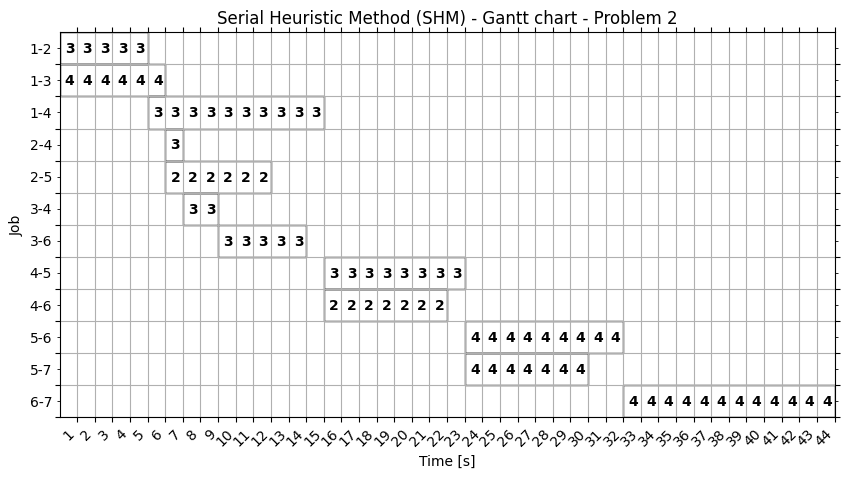
\includegraphics[width=0.8\linewidth]{images/comparison/shm_problem_2.png}
	\caption{Timeline of the activities in problem 2 as scheduled by SHM.
		The vertical axis represents the job, while the horizontal axis displays the time in seconds.
		The numbers in the squares represent the CPU cores required by each job at a point in time.
	}
	\label{Figure:comparison->problem->2->timelines->shm}
\end{figure}

\begin{figure}[ht!]
	\centering
	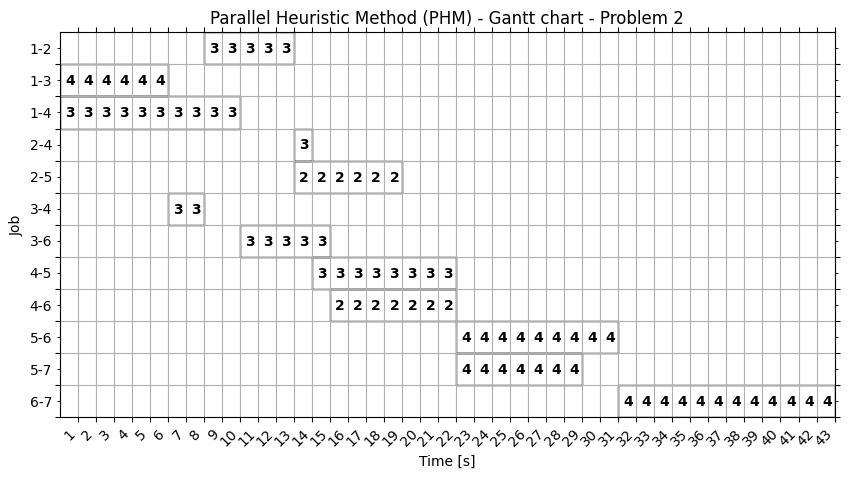
\includegraphics[width=0.8\linewidth]{images/comparison/phm_problem_2.png}
	\caption{Timeline of the activities in problem 2 as scheduled by PHM.}
	\label{Figure:comparison->problem->2->timelines->phm}
\end{figure}

\begin{figure}[ht!]
	\centering
	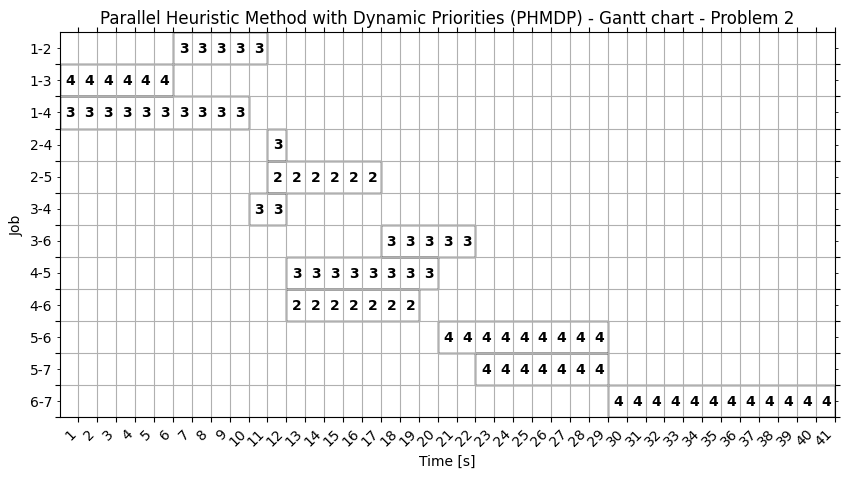
\includegraphics[width=0.8\linewidth]{images/comparison/phmdp_problem_2.png}
	\caption{Timeline of the activities in problem 2 as scheduled by PHMDP.}
	\label{Figure:comparison->problem->2->timelines->phmdp}
\end{figure}

\subsection{Problem 3}
The visualization of problem 3 as a CPM network is shown in Figure~\ref{Figure:comparion->problem->3->cpm-network}. For this problem, $r_\mathrm{max}$ was set to 6.

\begin{figure}[ht!]
	\centering
	\begin{tikzpicture}[
		mynode/.style={
			circle,
			draw=black,
			fill=gray,
			fill opacity = 0.3,
			text opacity=1,
			inner sep=0pt,
			minimum size=20pt,
			font=\small},
		myarrow/.style={-Stealth},
		node distance=0.6cm and 1.2cm
		]
		\node[mynode] (n1) {1};
		\node[mynode,above right=of n1] (n2) {2};
		\node[mynode,below=of n2] (n3) {3};
		\node[mynode,below=of n3] (n4) {4};
		\node[mynode,right=of n2] (n5) {5};
		\node[mynode,right=of n5] (n7) {7};
		\node[mynode,below=of n7] (n6) {6};
		
		
		\foreach \i/\j/\txt/\p in {% start node/end node/text/position
			n1/n2/{4, 3}/above,
			n1/n3/{3, 4}/above,
			n1/n4/{5, 3}/above,
			n2/n5/{3, 2}/above,
			n3/n5/{2, 3}/above,
			n4/n6/{4, 2}/below,
			n5/n6/{3, 4}/above,
			n5/n7/{4, 3}/above}
		\draw [myarrow] (\i) -- node[sloped,font=\small,\p] {\txt} (\j);
		
	\end{tikzpicture}
	\caption{Visualization of problem 3 as a CPM network.
		Each weighted edge represents a job, its duration (in seconds), and the number of CPU cores required.
	}
	\label{Figure:comparion->problem->3->cpm-network}
\end{figure}

The timelines produced by SHM, PHM, and PHMDP are shown in Figures~\ref{Figure:comparison->problem->3->timelines->shm}, \ref{Figure:comparison->problem->3->timelines->phm}, and \ref{Figure:comparison->problem->3->timelines->phmdp}, respectively.
In the case of problem 3, PHM and PHDMP tied in scheduling the jobs to complete in the shortest time: 17 seconds.
However, SHM was only two seconds behind.

\begin{figure}[ht!]
	\centering
	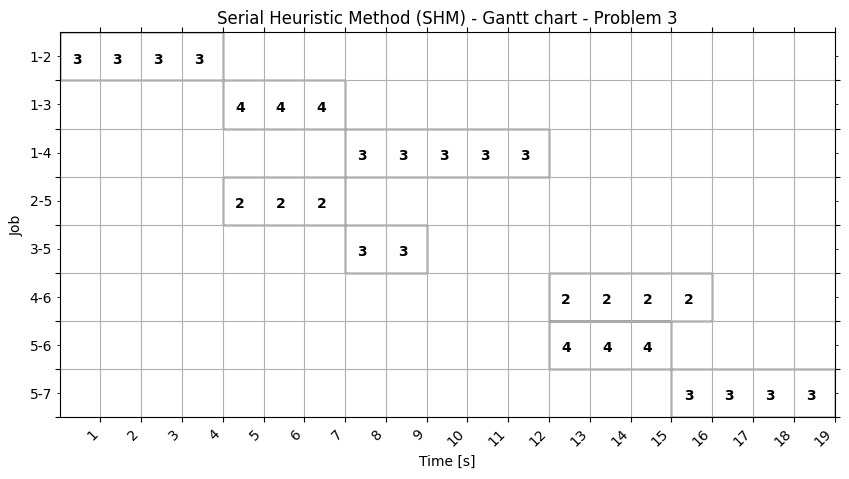
\includegraphics[width=0.8\linewidth]{images/comparison/shm_problem_3.png}
	\caption{Timeline of the activities in problem 3 as scheduled by SHM.
		The vertical axis represents the job, while the horizontal axis displays the time in seconds.
		The numbers in the squares represent the CPU cores required by each job at a point in time.
	}
	\label{Figure:comparison->problem->3->timelines->shm}
\end{figure}

\begin{figure}[ht!]
	\centering
	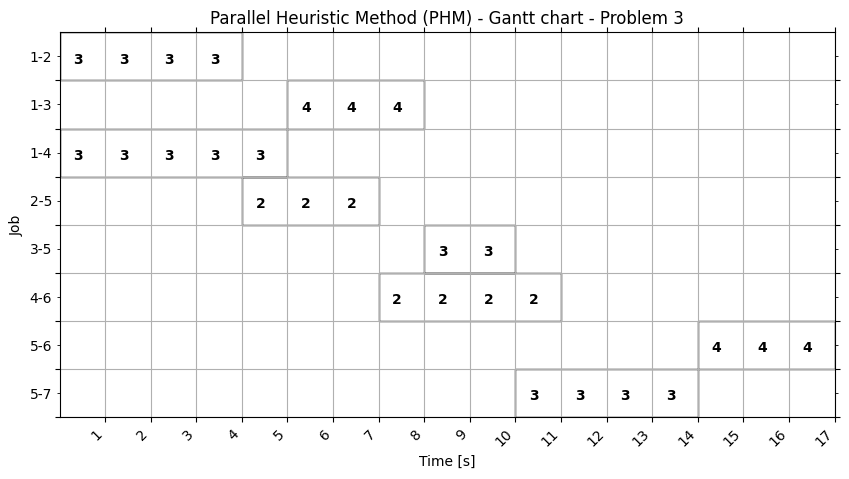
\includegraphics[width=0.8\linewidth]{images/comparison/phm_problem_3.png}
	\caption{Timeline of the activities in problem 3 as scheduled by PHM.}
	\label{Figure:comparison->problem->3->timelines->phm}
\end{figure}

\begin{figure}[ht!]
	\centering
	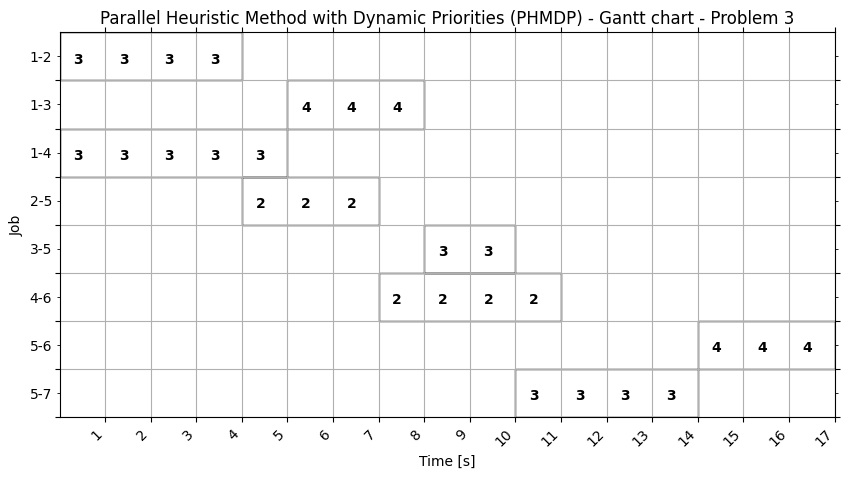
\includegraphics[width=0.8\linewidth]{images/comparison/phmdp_problem_3.png}
	\caption{Timeline of the activities in problem 3 as scheduled by PHMDP.}
	\label{Figure:comparison->problem->3->timelines->phmdp}
\end{figure}

\section{Conclusion}

\printbibliography

\nocite{*}

\end{document}